\documentclass{article}
\usepackage[a4paper, margin=2cm]{geometry}

\usepackage{amsmath}
\usepackage{amssymb}
\usepackage{mathtools}
\usepackage{amstext}
\usepackage{amsthm}
\usepackage{fancyhdr}
\usepackage{siunitx}
\usepackage{physics}

\usepackage{hyperref}

\usepackage{tikz}
\usetikzlibrary{patterns}
\usepackage{pgfplots}
\usetikzlibrary{arrows}
\usetikzlibrary{decorations.pathreplacing}



\usepackage{graphicx}
\usepackage{float}
\graphicspath{{figures/}} %Setting the graphicspath
\usepackage{float}
\usepackage{caption}
\usepackage{subcaption}
\usepackage{booktabs}

% To work with inkfigures
\usepackage{import}
\usepackage{pdfpages}
\usepackage{transparent}
\usepackage{xcolor}

\newcommand{\incfig}[2][1]{%
    \def\svgwidth{#1\columnwidth}
    \import{./figures/}{#2.pdf_tex}
}

\pdfsuppresswarningpagegroup=1

%\graphicspath{{figures/}}

\pagestyle{fancy}
\rhead{Alexandre Adam}
\lhead{PHY6669 -- Cosmologie \\ Alan Robinson}
\chead{Devoir 2}
\rfoot{\today}
\cfoot{\thepage}

\newcommand{\angstrom}{\textup{\AA}}
\numberwithin{equation}{section}
\renewcommand\thesubsection{\alph{subsection})}
\renewcommand\thesubsubsection{\Roman{subsubsection}}
\newcommand{\s}{\hspace{0.1cm}}

\newcommand{\pyoutput}[2]{#2}

% Astronomy
\DeclareSIUnit\parsec{pc}
\DeclareSIUnit\lightyear{ly}
%\usepackage[backend=bibtex,bibencoding=ascii,style=authoryear,sorting=none]{biblatex}
%\usepackage{biblatex}
%\addbibresource{bibfile.bib}



\begin{document}
\section{Les distances en cosmologie}
\subsection{Distance angulaire}
On cherche le redshift $z$ où l'angle apparent d'un objet est à son minimum en supposant 
un univers dominé par la matière.

L'angle apparent d'un objet dépend de la taille que cette objet aurait au 
temps présent ($\ell(z)$) et de la distance 
comobile entre l'observateur et l'objet:
\begin{equation}\label{eq:AngleApparent} 
        \theta = \frac{\ell(z)}{\chi(z)}
\end{equation} 
Un objet de taille caractéristique $\ell$ (dans son référentiel, au temps 
où l'objet à émis la lumière observée) aura une taille assumée dans le référentiel 
de l'observateur égale à
\[
        \ell(z) = \frac{a_0}{a}\ell = (1 + z) \ell
\]
Pour un univers de poussière ($\Lambda = p = 0$), la distance comobile prend une forme 
analytique:
\begin{equation}\label{eq:ComovingDistanceDust} 
        \chi(z) = \frac{2 c}{H_0} \frac{\Omega_0 z + (\Omega_0 - 2)
        (\sqrt{\Omega_0 z + 1} - 1)}{\Omega_0^2(1 + z)}
\end{equation}
On peut donc déterminer un redshift où la taille atteint un maxima:
\begin{align*}
        \frac{d \theta}{d z} &= \frac{H_0 \ell}{2c} \frac{d }{d z} 
                \frac{\Omega_0^2(1 + z)^2}{\Omega_0 z + (\Omega_0 - 2) 
                (\sqrt{\Omega_0 z + 1} - 1)} \\
        &= \frac{\Omega_0^2 H_0 \ell}{2c} 
                \frac{2(1 + z) \left[ \Omega_0 z + (\Omega_0 - 2) 
                (\sqrt{\Omega_0 z + 1} - 1) \right] - 
        (1 + z)^{2} \left[ \Omega_0 + 
        \frac{1}{2}\frac{\Omega_0(\Omega_0 - 2) }{\sqrt{\Omega_0 z  + 1}}\right]}{
        (\Omega_0 z + (\Omega_0 - 2)(\sqrt{\Omega_0 z + 1} - 1))^{2}        
}
\end{align*}
Il s'avère qu'il est possible de résoudre analytiquement 
ce système seulement pour $\Omega_0 = 1$ (univers plat):
\begin{align*}
        \frac{d \theta}{d z}\bigg|_{\Omega_0=1} &= 0 \\
        \implies 2\left[ z -\sqrt{z + 1} + 1\right]
        &= (1 + z) \left[ 1 - \frac{1}{2\sqrt{z + 1}} \right] \\
        \implies 2(x^2 - x) &=  x^2(1 - \frac{1}{2x}), \hspace{1cm} \{x = \sqrt{z + 1} \} \\
        \implies x^2 - \frac{3x}{2} &=  0 \\
        \implies \sqrt{z + 1} &= \frac{3}{2}, \hspace{2.5cm} \{ z \geq 0 \implies x \not= 0 \} \\
        \implies \Aboxed{z &=  \frac{5}{4}}
\end{align*}
Il serait possible de faire un traitement perturbatoire pour $\Omega_0 = 1 \pm \epsilon$, 
$\epsilon \ll 1$, mais on trouve qu'une solution numérique sert mieux nos besoins. 
Les prochaines figures montrent le redshift où l'angle apparent est minimal pour une 
une densité totale $\Omega_0$ donnée.

\begin{figure}[H]
        \centering
        \begin{subfigure}[t]{0.52\textwidth}
                \includegraphics[width=\textwidth]{theta_z}
                \caption{Taille angulaire apparente d'un objet de distance 
                caractéristique $\ell$}
                \label{fig:theta_z}
        \end{subfigure}
        ~
        \begin{subfigure}[t]{0.45\textwidth}
                \includegraphics[width=\textwidth]{zmin} 
                \caption{Le redshift où $\theta$ est minimal
                        se comporte comme $\Omega_0^{-1}$ autour 
                        de la solution pour un univers plat.}
                \label{}
        \end{subfigure}
\end{figure}

\subsection{Le nombre total de galaxies dans l'univers}
Pour déterminer la densité de galaxie de l'univers à un temps donné, il est coutume de 
se référer à la fonction de Schechter pour mesurer la densité numérique de galaxies 
en fonction de leur distribution de masse:
\begin{equation}\label{eq:Schechter} 
        \phi(M) = b\phi^* \ln(10) \left[ 10^{b(M - M^{*})} \right]^{1 + \alpha} \exp \left\{ 
        -10^{b(M - M^{*})}\right\}
\end{equation} 
où $b=1$ pour la fonction de masse. En principe, $\alpha$, $M^{*}$ et $\phi^{*}$ doivent 
être ajusté sur les observations et peuvent dépendre de l'historique de formation 
des galaxies. En d'autres mots, ce sont des paramètres qui dépendent du redshift. On 
mesure $M$ en unité logarithmique de masse solaire:
\[
        M = \log \frac{M_{\text{gal}}}{M_\odot}
\]
La fonction de Schechter n'est valide que dans un interval de masses considérées. La borne 
inférieur choisie dans l'analyse de \cite{Conselice2016} est $M > 6$. Le meilleur fit sur les données 
pour la densité numérique intégrée sur le profile de Schechter $\phi_T$
\[
        \phi_T(z) = \int_{M_1}^{M_2} \phi(M, z) dM \hspace{0.5cm} [\text{Mpc}^{-3}]
\]
est \cite{Conselice2016}
\[
        \log \phi_T(t) = (-1.08 \pm 0.20) \log \left( \frac{t}{1\, \text{Gyr}} \right) - 0.26 \pm 0.06
\]
Ce résultat est un constat que le taux de production de galaxies est variable 
en fonction du temps. En particulier, il est plus bas aujourd'hui qu'il ne l'était 
à $z=6$.

Le nombre total de galaxies dans l'univers visible, 
en supposant un modèle d'évolution
qui commence à $z = 6$ et la cosmologie du modèle $\Lambda \text{CDM}$ plat, est 
donc l'intégrale de la fonction du nombre de densité total multiplié par 
le volume de l'univers visible en fonction du redshift $V_{\text{univers}}(z)$:
\begin{equation}\label{eq:NtotGal} 
        N_{\text{tot}} = \frac{c}{H_0} \int_{z=0}^{6} 
        \int_0^{4 \pi} 
        \underbrace{\frac{(1 + z)^{2} D_A^{2}}{
        \sqrt{\Omega_{0m}(1 + z)^{3} + \Omega_{0\Lambda}}}}_{
\dfrac{\partial^{2} V_{\text{univers}}(z)}{\partial \Omega \partial z}}
        \phi_T(t(z)) d\Omega dz
\end{equation} 
où $D_A$ est la distance angulaire en fonction de $z$
\begin{equation}\label{eq:DA} 
        D_A(z) =  \frac{(1 + z)^{-1}}{H_0}\int_0^{z} \frac{dz'}{\sqrt{\Omega_{0m}(1 + z')^{3} 
        + \Omega_{0\Lambda}}}
\end{equation} 
et
\begin{equation}\label{eq:t(z)} 
        t(z) = \frac{1}{H_0}\int_z^{\infty } \frac{(1 + z')^{-1} dz'}{
        \sqrt{\Omega_{0m}(1 + z')^{3} + \Omega_{0\Lambda}}}
\end{equation} 
Les paramètres du modèle cosmologique sont données dans la table suivante.
\begin{table}[H]
        \centering
        \begin{tabular}{ccc}
                \toprule
                $h$ & $\Omega_{0m}$ & $\Omega_\Lambda$ \\
                0.7 & 0.3 & 0.7 \\
                \bottomrule
                
        \end{tabular}
        \caption{}
        \label{tab:}
\end{table}
Le résultat de l'équation \eqref{eq:NtotGal} est 
\[
        \boxed{N_{\text{tot}} = (6 \pm 1) \times 10^{11}\, \text{galaxies}}
\]
%En principe, il y a $N_{\text{tot}}$ galaxie observable dans l'univers visible.


\section{L'horizon}
L'horizon comobile est définie comme
\[
        \eta \equiv \int_0^t \frac{dt'}{a(t')}
\]
$(c = 1)$. La distance comobile entre deux points est définie comme
\[
        \chi(a) = \int_a^{1} \frac{da'}{a'^2 H(a')}
\]

\subsection{}\label{sec:2a}
On cherche le redshift à partir duquel un miroir peut réfléchit la lumière du Big Bang 
vers la position d'un observateur de sortes que celui-ci reçoit cette lumière au temps 
$t_0$.
\begin{figure}[H]
        \centering
        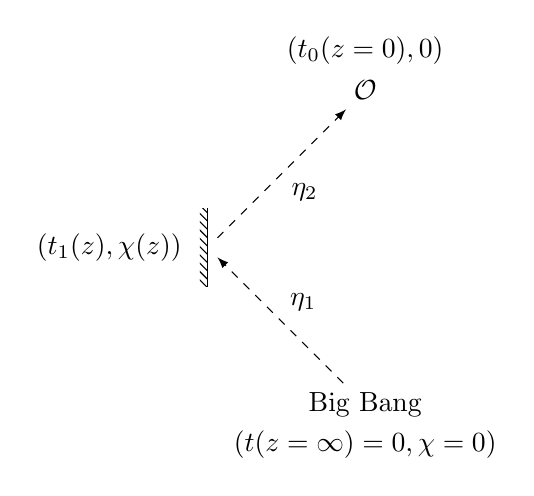
\begin{tikzpicture}
                \node (bb) at (0, 0) {Big Bang};
                \node at (0, -0.5) {$(t(z=\infty) = 0, \chi=0)$};
                \node (miroir) at (-2, 2) {};
                \node at (-3.25, 2) {$(t_1(z), \chi(z))$};
                \draw (-2, 1.5) -- (-2, 2.5); 
                \draw[pattern=north west lines, draw=none] (-2, 1.5) rectangle (-2.1, 2.5);
                \node (obs) at (0, 4) {$\mathcal{O}$};
                \node at (0, 4.5) {$(t_0(z=0), 0)$};
                \draw[-latex, dashed] (bb) -- (miroir) node [midway, above right] {$\eta_1$};
                \draw[-latex, dashed] (miroir) -- (obs) node [midway, below right] {$\eta_2$};
                %\draw[decorate, decoration={brace, amplitude=5pt, mirror}, xshift=0pt, yshift=0pt] 
                        %(-2, -1) -- (0, -1);
                %\node at (-1, -1.5) {$\chi(z)$};
        \end{tikzpicture}
        \caption{Illustration du problème}
        \label{fig:Numero2a}
\end{figure}

Par géométrie, les horizons comobiles $\eta_1$ et $\eta_2$ sont égales à la distance 
comobile $\chi(z)$ entre le miroir et l'observateur:
\[
        \chi(z) = \frac{1}{2} \left( \int_0^{t_1} \frac{dt}{a(t)} 
        + \int_{t_1}^{t_0} \frac{dt}{a(t)}\right)
\]
Pour un univers de poussière ($\Lambda=p=0$) plat ($\Omega_0=1$), les équations de 
Friedmann ont comme solution
\begin{align*}
        t(z) &=  t_0 (1 + z)^{-3/2} \\
        \implies dt &= -\frac{3}{2}t_0 (1 + z)^{-5/2}dz
\end{align*}
En remplaçant $a(z) = (1 + z)^{-1}$, dans l'intégrale de l'horizon comobile, on obtient
\[
        \chi(z) = \frac{1}{2} \int_\infty^{0} \left( - \frac{3}{2} \right)t_0
        (1 + z)^{-3/2} dz
\]
Ainsi,
\[
        \chi(z) = \frac{3}{2H_0}
\]
Du côté gauche, la distance comobile prend la forme
\[
        \chi(z) = \frac{2}{H_0}\left( 1 - \frac{1}{\sqrt{1 + z}} \right)      
\]
De sortes que 
\begin{align*}
        1 - \frac{1}{\sqrt{1 + z}} &=  \frac{3}{4} \\
        \implies \Aboxed{z &= 3} 
\end{align*}



\subsection{}
Dans un univers ouvert ($\kappa  = -1, \Omega < 1$) 
dominé par la matière ($\Lambda = p = 0$), les équations de Friedmann deviennent
\begin{align*}
        \dot{a}^{2} &=  \frac{8 \pi G \rho a^2}{3} + 1 \\
        \ddot{a} &=  -\frac{4\pi G \rho a}{3} \\
        d(\rho a^3) &=  0
\end{align*}
On introduit le paramètre de densité au temps présent 
\[
        \Omega_0 = \frac{\rho_0}{\rho_{0c}}, \hspace{1cm} \rho_{0c} = \frac{3H_0^2}{8 \pi G}
\]
En utilisant notre équation d'état, on peut remplacer $\rho a^{3} = \rho_0 a_0^{3}$:
\begin{align*}
        \implies \left( \frac{\dot{a}}{a_0} \right)^{2} 
        &= H_0^{2}\Omega_0 \frac{a_0}{a}  + \frac{1}{a_0^{2}} \\
\end{align*}
On remarque que le terme $1/a_0^2$ est constant. On peut ainsi, en manipulant 
l'équation, le remplacer en terme des constantes physiques actuelles:
\[
        \left( \frac{\dot{a}}{a_0} \right)^{2} - H_0^2 \Omega_0 \frac{a_0}{a} = \frac{1}{a_0^2}
\]
En particulier, cette équation est vrai à $a = a_0$, donc on obtient
\begin{equation}\label{eq:FriedDustOuvert} 
        \left( \frac{\dot{a}}{a_0} \right)^{2} 
        = H_0^{2} \left( \Omega_0 \left( \frac{a_0}{a}\right) + (1 - \Omega_0)  \right)
\end{equation} 
On remarque premièrement que $\dot{a} > 0\, \forall\, t$, puisque le côté droit 
de l'équation est toujours positif pour un univers ouvert ($\Omega_0 < 1$).
Ainsi, on s'attend que le facteur d'échelle 
augmente en fonction de $t$ et que $\Omega_0 a_0 /a$ devienne négligeable 
devant $1 - \Omega_0$ à un certain moment dans l'évolution de l'univers.

Ceci survient lorsque 
\[
        a \gg a^* = \frac{a_0\Omega_0}{1 - \Omega_0}
\]
Ainsi,
%Pour $\Omega_0 \simeq 0$, le premier terme va devenir néglige
\begin{align*}
        \dot{a} &\simeq H_0 (1 - \Omega_0)^{1/2} \\
        \implies \Aboxed{a(t) &\simeq H_0 (1 - \Omega_0)^{1/2} t,\,\,\, a \gg a^*}
\end{align*}

\subsection{}
Pour répéter l'expérience de pensée de la sous section \ref{sec:2a}, on doit déterminer 
la solution $a(t)$ générale. On définit le temps conforme $\eta$ de sortes que 
\[
        d\eta = H_0\sqrt{1 - \Omega_0}\frac{dt}{a}
\]
Ainsi,
\[
        \frac{1}{H_0 \sqrt{1 - \Omega_0}} \left( \frac{\dot{a}}{a_0} \right) =
        \frac{1}{a_0 H_0 \sqrt{1 - \Omega_0}} \frac{da}{dt} = \frac{1}{a_0}\frac{d \ln a}{d\eta} 
\]
On intègre l'équation de Friedmann en terme du temps conforme avec la condition 
initiale $a(\eta = 0) = 0$ et $a_0 = 1$:
\[
        \eta = 
        \int_0^{a} \frac{d a'}{ \sqrt{\dfrac{\Omega_0}{1 - \Omega_0} a' + a'^2}}
\]
Cette intégrale a une primitive en terme du logarithme naturel:
\[
        \eta = 
        \ln \left( \frac{\frac{1}{2}\frac{\Omega_0}{1 - \Omega_0}  + a
                        + \sqrt{\frac{\Omega_0}{1 - \Omega_0} a + a^2}
        }{\frac{1}{2}\frac{\Omega_0}{1 -\Omega_0}} \right)
\]
Notons que
\[
        \cosh^{-1}(x) = \ln(x + \sqrt{x^{2} - 1})
\]
Ainsi,
\[
        \eta = 
        \cosh^{-1} \left( 1 + \frac{2a(1 - \Omega_0)}{\Omega_0} \right)
\]
D'où on trouve que 
\begin{equation}\label{eq:Ahyperbolic} 
        a(\eta) = \frac{1}{2} \frac{\Omega_0}{1 - \Omega_0}(\cosh (\eta) - 1)
\end{equation} 
Similairement, on trouve (avec $t(0) = 0$):
\begin{equation}\label{eq:thyperbolic} 
        t(\eta) =\frac{1}{H_0 \sqrt{1 - \Omega_0}} \int_0^{\eta}a(\eta')d\eta' = \frac{1}{2}\frac{\Omega_0}{
        H_0(1 - \Omega_0)^{3/2}} (\sinh(\eta) - \eta) 
\end{equation} 

Notons qu'on a utiliser la variable $\eta$ pour représenter le temps conforme, car ce temps 
correspond aussi à l'horizon cosmique définit plus haut (multiplié par le bon facteur). 
Il est facile de le démontrer 
avec les équations différentielles définit plus haut. La distance comobile est simplement
\[
        \eta_{\text{horizon}} = \frac{c}{H_0 \sqrt{1 - \Omega_0}} \eta
\]
\[
        \chi(\eta) = \frac{c}{H_0 \sqrt{1 - \Omega_0}} (\eta_0 - \eta)
\]
où $\eta_0$ correspond au temps conforme présent. Le problème du miroir revient donc à résoudre 
\[
        \frac{1}{1 + z} = a(\eta = \frac{1}{2}\eta_0)
\]
On trouve $\eta_0$ par l'équation \eqref{eq:Ahyperbolic} ($a_0 = 1$):
\[
        \eta_0 = \cosh^{-1} \left( \frac{2 - \Omega_0}{ \Omega_0} \right)
\]

\begin{figure}[H]
        \centering
        \includegraphics[width=0.45\textwidth]{numero2c_sol}
        \caption{On remarque que la solution diverge lorsque $\Omega_0 \rightarrow 0$, 
        ce qui attendu. La solution converge aussi vers la solution d'un 
univers plat développé à la sous-section \ref{sec:2a}.}
        \label{fig:z_miroir}
\end{figure}

%On peut donc exprimer l'horizon comobile entre des expressions trouvées pour $a(\xi)$ et 
%$t(\xi)$. Notons que 


\section{Le signal de EDGES}
Le téléscope radio EDGES a mesuré la température de transition hyperfine 
de l'hydrogène dans l'interval $13 < z < 27$. Un abaissement de la température 
du spin de l'hydrogène est attendu entre $z=20$ et $z=15$, au moment où les 
première étoiles commencent à rayonner et exciter l'état triplet de l'hydrogène.

\subsection{Ratio de température}
La température du rayonnement évolue comme
\[
        T_\gamma = T_{\text{CMB}}(1 + z)
\]
Alors que la température du gaz évolue plutôt comme
\[
        T_{\text{gaz}} = T_0(1 + z)^{2}
\]
En utilisant le fait que $T_{gaz}(z=200) \simeq T_\gamma(200)$, on peut 
déterminer $T_0$ et on trouve
\[
        \boxed{\frac{T_\gamma}{T_{\text{gaz}}} \simeq \frac{201}{21}}
\]
Ce qui correspond à une température
\[
        T_{\text{gaz}}(z=20) = 5.97\, \text{K}
\]

\subsection{}
La température du profil d'absorption $T_{21}$ suit la loi
\[
        T_{21} = \frac{1}{1 + z}(T_s - T_{\text{CMB}})(1 - e^{-\tau})
\]
où $\tau$ est l'épaisseur optique à l'époque de la réionization et $T_s$ est la 
température du spin de l'hydrogène. Plus précisément, c'est la température 
effective qui mesure le ratio d'hydrogène dans l'état singulet (1) et l'état 
triplet (2) par la distribution de Boltzmann:
\begin{equation}\label{eq:Tspin} 
       \frac{n_2}{n_1} = \frac{g_2}{g_1}\exp \left\{ -\frac{E_{21}}{k_bT_s} \right\} 
\end{equation} 
%Avec le modèle de la section précédente, en assumant $T_{\text{gaz}} = T_s$ et 
%en prenant $\tau = 0.066 \pm 0.012$ , on trouve \cite{}
En assumant que l'épaisseur optique est $\tau \ll 1$, on trouve \cite{Madau1996}
\begin{equation}\label{eq:Tedges} 
        T_{21} \simeq (0.011\, \text{K})\frac{2}{h}\left( \frac{\Omega_b h^2}{0.2} \right)
        \sqrt{\frac{1 + z}{9}} x_{HI} \left( \frac{T_S - T_\gamma}{T_S} \right)
\end{equation} 
où $T_S$ est la température de spin de l'hydrogène et $x_{HI}$. On suppose $T_{\text{gaz}} = T_S$ 
et $x_{HI} \simeq 1$.
Le résultat de EDGES montre que $\delta T\simeq -500\, \text{mK}$. On infère la 
température du gaz en inversant la relation \ref{eq:Tedges} pour déterminer 
\[
        T_S(z=20) \simeq 0.62\, \text{K}
\]
Ce résultat confirme que la température de l'hydrogène qui est responsable 
du signal mesuré par EDGES est beaucoup plus petite que celle à laquelle on 
s'attend ($5.97\, \text{K}$). On peut construire un modèle où une certaine 
quantité de matière noire $\chi$ très froide interagit avec le bain d'hydrogène 
pour le refroidir. Dans ce cas,
\[
        \frac{T_{S}(z = 20)}{T_{\text{gaz}}(z=20)} = \frac{n_H}{n_H + n_\chi}
\]
Ainsi, en utilisant les résultats de la collaboration Planck \cite{PlanckCollaboration2018}:
\[
        \boxed{n_\chi = n_h \left( \frac{T_{\text{gaz}}}{T_S} - 1 \right) 
        \simeq  0.014\, \text{cm}^{-3}}
\]
où $n_H \simeq 1.62\times 10^{-3}\, \text{cm}^{-3}$.

\bibliography{bibfile.bib}
\bibliographystyle{abbrv}




\end{document}

